\begin{frame}
  \frametitle{Customize your board device tree!}
  \small
  Often needed for embedded board users:
  \begin{columns}
    \column{0.65\textwidth}
       \begin{itemize}
       \item To describe external devices attached to non-discoverable
             busses (such as I2C) and configure them.
       \item To configure pin muxing: choosing what SoC signals are
	     made available on the board external connectors.
	     See \url{http://linux.tanzilli.com/} for a web service doing this
	     interactively.
       \item To configure some system parameters: flash partitions,
	     kernel command line (other ways exist)
       \item Device Tree 101 webinar, Thomas Petazzoni (2021):\\
             Slides: \url{https://bootlin.com/blog/device-tree-101-webinar-slides-and-videos/}\\
             Video: \url{https://youtu.be/a9CZ1Uk3OYQ}
       \end{itemize}
    \column{0.35\textwidth}
    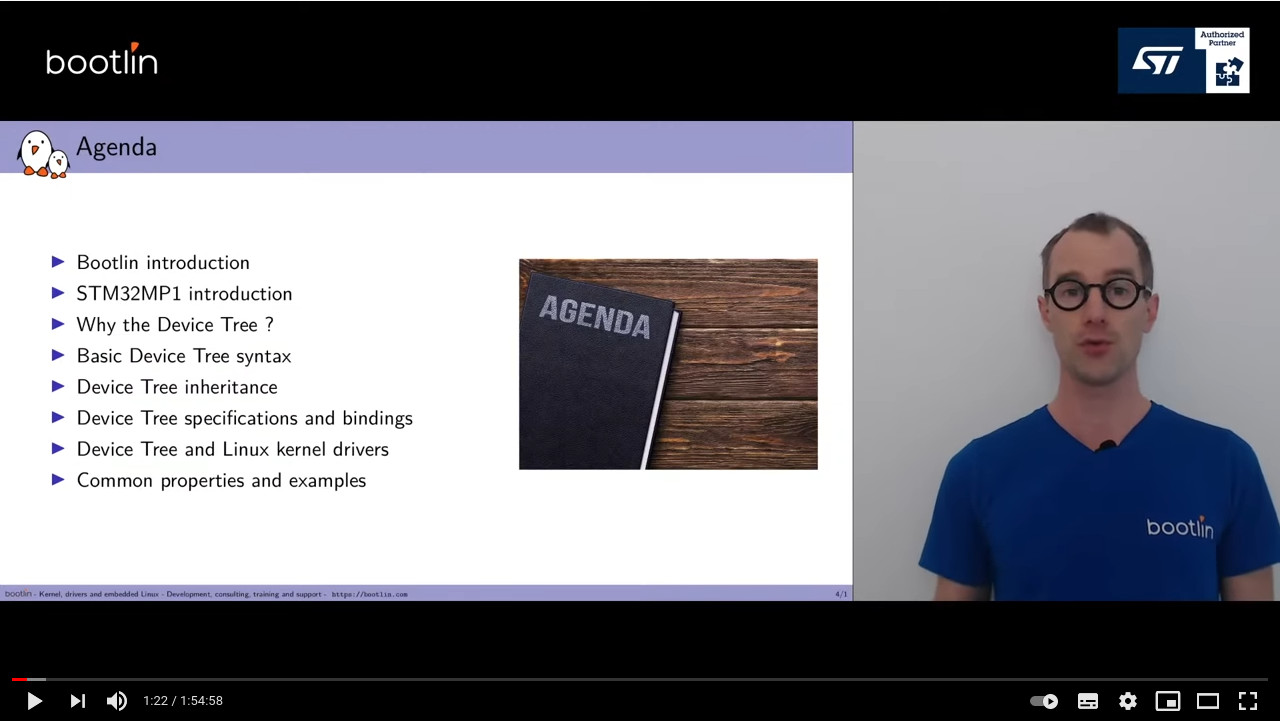
\includegraphics[width=\textwidth]{common/device-tree-video.jpg}
  \end{columns}
\end{frame}
